\chapter{Desenvolvimento do tema}
\label{cap:experiments}

Este capítulo é opcional e, a existir, é aqui que deve descrever como é que o seu projecto evoluiu.

O projeto é constituido em cinco partes:

\begin{enumerate}
    \item Ambiente de teste do projeto;
    \item Testes de FireWall e conexões realizados;
    \item \textit{"Port Controller"} - daemon em C\#;
    \item API e Interface Web;
    \item Sitema de notificações;
\end{enumerate}


No final o ambiente do projeto será o da seguinte imagem:

\begin{figure}[H]
\begin{center}
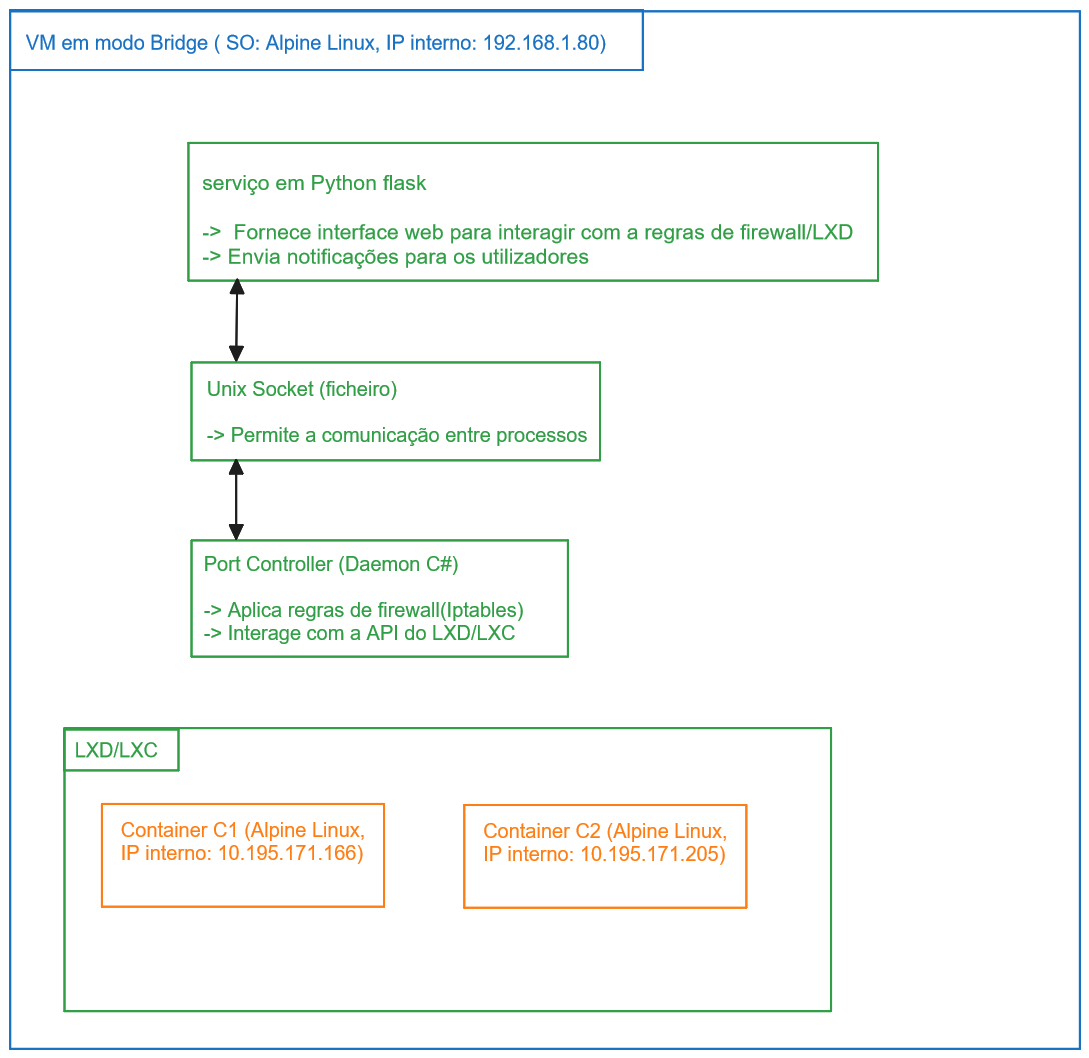
\includegraphics[width=14cm]{figs/estrutura2.png}
\caption{Abiente do projeto}
\label{fig:bookstack}
\end{center}
\end{figure}



\section{Ambiente de testes do projeto}

Esta secção do relatório irá abordar os passos efetuados na configuração do sistema 
usado como ambiente de testes do projeto e respetivas aplicações/pacotes instalados.

Sendo os seguintes:
\begin{enumerate}
    \item Configuração do Alpine Linux;
    \item Configuração do LXD/LXC;
    \item Instalação do .NET Core;
    \item Instalação de outros pacotes;
\end{enumerate}


\subsection{Configuração do Alpine Linux}

De modo a obter, os melhores resultados possiveis durate os estes e experiencias
ao longo deste projeto é de extrema importância que o sistema operativo de testes
seja o mesmo da plataforma Forge. Sendo assim foi intalada numa máquina virtual
VMware com o alpine linux 3.19.

Especificações atribuidas à maquina virtual:

\begin{itemize}
    \item 6 GB de RAM;
    \item 3 nucleos de para o CPU;
    \item Placa de rede no modo Bridge;
    \item 40 GB de armazenamento;
\end{itemize}

De seguida foi feita a configuração inicial do sistema com os seguintes coamandos:


\begin{enumerate}
    \item \texttt{localhost login: root 
    \item setup-alpine
    \item Select keyboard layout: pt-pt
    \item Enter a system hostname : alpine
    \item Which one do you want to initialize? [eth0]
    \item Ip address for eth0? [dhcp]
    \item Do you want to do any manual network configuration? (y/n) [n] n
    \item (Changing password for root) New password: ******
    \item which timezone are you in [UTC]
    \item HTTP/FTP proxy URL? [none]
    \item Enter mirror number (1-72) or URL to add (or r/f/e/done) [1]
    \item Setup user? (enter a lower-case loginname, or 'no') [no] delta
    \item Password: ******}
    \item Enter ssh key or URL for titus (or 'none') [none]
    \item Which ssh server ('openssh', 'dropbear', or 'none') [openssh]
    \item Which disk(s) would you like to use? [none] sda 
    \item how you would like to use it? ('sys', 'data', 'crypt', 'lvm' or '?'for help) [?] sys 
    \item Erase the above disk(s) and continue? (y/n) [n] y 
    \item Instalation Complete. Please reboot.
\end{enumerate}


\textbf{Nota:} As opcções \textit{default} são sugeridas dentro de "[]" caso se pretenda
usar essa opção é apenas necessário carregar na tecla "\textit{ENTER}". \\


Para terminar a configuração foi executado o comando: 

\texttt{apk add --upgrade apk-tools \&\& apk upgrade --available} \\


Foi também ativado o repositório da comunidae para ter um maior
numero de pacotes para instalar. Para isto é necessário descomentar a linha no
ficheiro "\textit{repositories}" com a localização "/etc/apk/repositories" com o
URL deste repositório, removendo o "\#" no inicio da linha.

No final o conteúdo do ficheiro deverá ser este:

\begin{lstlisting}[language=Bash, caption={Ficheiro repositories}]
http://dl-cdn.alpinelinux.org/alpine/v3.19/main
http://dl-cdn.alpinelinux.org/alpine/v3.19/community
\end{lstlisting}

\subsection{Configuração do LXD/LXC}

No que diz respeito ao LXD/LXC foram instalados os pacotes lxd e lxd-client.


Foi ativado o serviço do lxd como default com o comando \texttt{rc-update add lxd default}
e em seguida ativado com o \texttt{rc-service lxd start}.

Depois foi feita a configuração iniciul com o comando texttt{lxd init} com a seguintes opções:

\begin{enumerate}
    \item \texttt{Would you like to use LXD clustering? (yes/no) [default=no]: no
    \item Do you want to configure a new storage pool? (yes/no) [default=yes]: yes
    \item Name of the new storage pool [default=default]: default
    \item Name of the storage backend to use (btrfs, dir, lvm, zfs) [default=zfs]: dir
    \item Would you like to connect to a MAAS server? (yes/no) [default=no]: no;
    \item Would you like to create a new local network bridge? (yes/no) [default=yes]: yes
    \item What should the new bridge be called? [default=lxdbr0]: lxdbr0
    \item What IPv4 address should be used? (CIDR subnet notation, “auto” or “none”) [default=auto]: auto
    \item What IPv6 address should be used? (CIDR subnet notation, “auto” or “none”) [default=auto]: auto
    \item Would you like LXD to be available over the network? (yes/no) [default=no]: no
    \item Would you like stale cached images to be updated automatically? (yes/no) [default=yes] yes
    \item Would you like a YAML "lxd init" preseed to be printed? (yes/no) [default=no]: no}
\end{enumerate}

De seguida foi editada a configuração \textit{default} com o 
comando "\texttt{lxc profile edit default}" nela deverá ser garantida o
seguinte:

\begin{lstlisting}[language=csh, caption={edição do perfil padrão}]
  eth0:
    name: eth0
    nictype: bridged
    parent: lxdbr0
    type:nic

\end{lstlisting}

\textbf{Nota:} eth0 é a interface do sistema \textit{host} e lxdbr0 é a interface
de rede criada automaticamente pelo LXD.

Com esta configuração os \textit{containers} irão funcionar em modo NAT.


Após isto foram criados dois containers Alpine linux com o seguinte 
comando "\texttt{lxc launch images:alpine/3.19 <nome do container>}"

\begin{figure}[ht]
\begin{center}
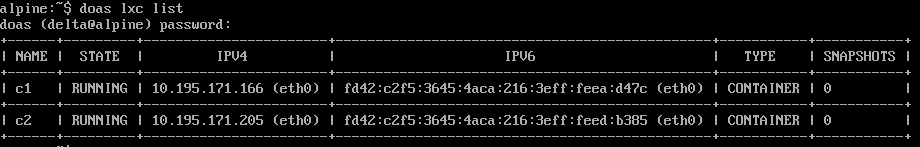
\includegraphics[width=14cm]{figs/lista de containers.png}
\caption{Containers criados.}
\label{fig:bookstack}
\end{center}
\end{figure}



\subsection{Instalação do .NET Core}


Para depois poder executar a aplicação que irá controlar as portas dos containers,
aplicação esta desenvolvida em C\# .NET Core é necessário instalar os pacotes necessários
para o funcionamento da mesma, mais concretamente o sdk e o \textit{runtime}.

Os pacotes necessŕios foram instalados usando os seguintes comandos:
\begin{itemize}
    \item \texttt{doas apk add dotnet7-sdk};
    \item \texttt{doas apk add dotnet7-runtime};
\end{itemize}




\subsection{Instalação de outros pacotes}

Para além do .NET Core, para garantir o funcionamento das aplicações desenvolvidas neste projeto é necessário
instalar ainda os seguintes pagotes:
\begin{itemize}
    \item Python - \texttt{doas apk add python3};
    \item Pip - \texttt{doas apk add python3-pip}
    \item Bash - \texttt{doas apk add bash};
\end{itemize}


Para uma maior facilidade de uso do sistema durante o seu uso foi também instalado
o "tmux" que permite criar "janelas" e trocar rapidamente entre as mesma, funcionalidade
essa que aumenta a produtividade num ambiente de apenas terminal.
Para asua instala ção foi usado o comando:
\begin{itemize}
    \item \texttt{doas apk add tmux};
\end{itemize}










\section{Testes de FireWall e conexões realizados}

Uma vez os \textit estarem configurados em modo NAT seria necessário criar regras 
de redirecionamento de portas ou endereços IP de modo a os \textit{containers} serem acedidos
por outros dispositivos na rede local.


De modo a realizar testes de conexão foram instalados dentro dos containers
o netcat e o python.

\textbf{Nota:} eth0 é a placa de rede do sistema host e tem o ip local de 192.168.1.80.


Durante os testes realizados, concluiu-se que existem três medodos de criar conectividade:

\subsection{Método 1: Criar regras no lxc network e defenir portas de redirecionamento}

\textbf{Nota:} Neste metodo será usado como exemplo o \textit{container} "c2" que
dentro da máquina virtual host tem o IP 10.195.171.166.

\textbf{Nota nº2:} A máquina virtual \textit{Host} tem o endereço IP 192.168.1.80.

Este metodo usa o comando "\texttt{lxc network forward create lxdbr0 192.168.1.80}"
para criar a regra e "\texttt{lxc network forward port add lxdbr0 192.168.1.80 tcp 7000 10.195.171.205 8000}"
para adicionar as portas a serem reencaminhadas, neste exemplo o trafego vindo da
rede local que tenta aceder ao endereço IP 192.168.1.80 (\textit{host}) pela porta 7000 será redirecionado
para a porta 8000 do IP 10.195.171.205 que pertence ao container "c2".

Nesta experiência o container está a executar um servidor http na porta 8000
com o comando "\texttt{python3 -m http.server}".


\textbf{Nota:} Porta 8000 é a padrão quando não é especificada outra no final do comando.


Foi possivel aceder ao servidor HTTP pelo browser num computador da rede local.

\begin{figure}[H]
\begin{center}
\includegraphics[width=12cm]{figs/teste de conexão via browser.png}
\caption{Teste de conexão via browser.}
\label{fig:bookstack}
\end{center}
\end{figure}


Foram também usados alguns comandos do netcat como o "\texttt{nc -w1 -vz 192.168.1.80 7000}".

\begin{figure}[ht]
\begin{center}
\includegraphics[width=12cm]{figs/teste de conexão1.png}
\caption{Teste de conexão com o netcat.}
\label{fig:bookstack}
\end{center}
\end{figure}

Foram usados também usados os comandos "\texttt{nc 192.168.1.80 7000} e \texttt{nc -l 8000}"
de modo a criar uma ligação TCP. Foi também testado a ligação reversa
onde o \textit{container} se tenta ligar ao computador da rede, invertendo os comandos
"\texttt{nc 192.168.1.68 3000}" e "\texttt{nc -l 3000}", ambos os testes foram bem
sucedidos.







\subsection{Método 2: Usar um IP para redirecionar o tráfego para o container}

Neste método é atribuido um endereço ip da rede local, que esteja disponivel, à
interface de rede do sistema host, eth0, usado o comando
"\texttt{ip address add 192.168.1.120/24 dev eth0}", para este exemplo foi escolhido o IP
"192.168.1.120".

De seguida, é necessário criar a regra de redirecionamento do tráfego
com o IP de destino "192.168.1.120" para o IP de um \textit{container}, que neste esxemplo será o
IP "10.195.171.166" que pertence ao \textit{container} "c1", para isto foi usado o
comando "\texttt{lxc network forward create lxdbr0 192.168.1.120 target\_address=10.195.171.166}"
que automaticamente cria uma regra na tabela NAT do iptables para garantir o correto
funcionamento do redirecionamento.

Com esta configuração se o \textit{container} "c1" que possui o IP "10.195.171.166" estiver a executar um servidor 
http na porta 8000, o mesmo serviço estará disponivel para dispositivos da rede local
através do IP 192.168.1.120 na porta 8000.

\textbf{Nota:} Os testes de conexão usados no método 1 foram igualmente bem sucedidos.

\subsection{Método 3: Usar o Iptables para criar portas de redirecionamento}

O método 3 é o mesmo que o médoto 1 mas só que configurado usando apenas regras
do Iptables, ou seja, é criaca uma regra na tablea NAT que redireciona o tráfego
de uma porta do sistema host para um IP e porta de um \textit{container}.

É possivel criar esta configuração com o comando:



\begin{lstlisting}[language=Bash, caption={Exemplo de regra de redirecionamento}]
    doas iptables -t nat -I PREROUTING -p tcp --dport 5000 -j DNAT --to-destination 10.195.171.205:8000
\end{lstlisting}



Neste exemplo similar ao exemplo di método 1, se o \textit{container} "c2" com o 
endereço IP "10.195.171.205", estiver a executar um servidor HTTP na porta
8000, os dispositivos na rede local poderão aceder a este serviço acedendo à porta 
5000 do IP do sistema host(192.168.1.80).

\textbf{Nota:} Os testes de conexão usados no método 1/2 foram igualmente bem sucedidos.


% =============================================================================


\section{Criação da API}

Para interagir com o daemon C\# (Port Controller) responsável por interagir com regras do iptables
e configurações do LXC/LXD, foi criada uma API em Python com a biblioteca Flask como
método alternativo à interface \textit{Web}.

O principal motivo da criação desta API é a facilitação nos momentos de teste dos programas
desenvolvidos, uma vez que pode ser testada no terminal com o comando Curl. Contudo, nada 
impede o administrador do sistema de usar este método de interação com o "Port Controler"
como forma principal, uma vez que funciona de formna independente da interface Web.

Sendo assim, neste componente do projeto desenvolvida em Python à três partes essencias:

\begin{enumerate}
    \item API - que permite ao utilizador (administrador do sistema) interagir com o "Port Controller" daemon em C\#
    através do terminal fazendo solicitações HTTP com o comando Curl;
    \item Interface Web - que permite ao utilizador (administrador do sistema) interagir com o "Port Controller"
    através de uma interface gráfica que pode ser acedida através do \textit{browser};
    \item O ficheiro que comunica com a unix socket (localizada em /tmp/socket\_proj) que por sua vez, comunica com o "Port Controller". 
\end{enumerate}

Nesta secção o foco será a explicação do funcionamento da API, porém, para esclarecer
melhor o funcionamentodos ficheiros referidos a seguinte imagem mostra o fluxo de comunicação
entre os ficheiros/programas do projeto.

\begin{figure}[H]
\begin{center}
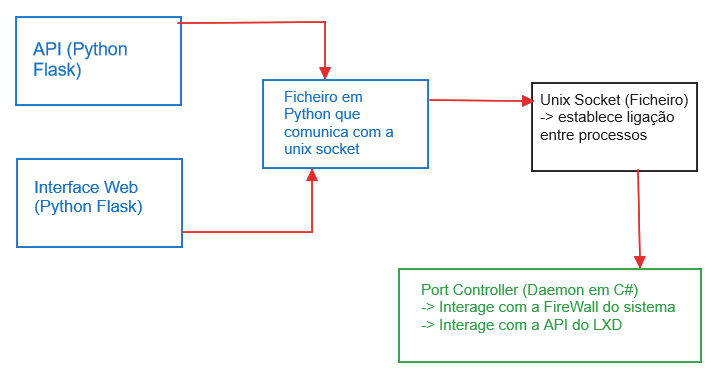
\includegraphics[width=14cm]{figs/fluxo de comunicação.png}
\caption{Fluxo de comunicação do projeto}
\label{fig:bookstack}
\end{center}
\end{figure}

\subsection{Estrutura da API}

A API está dividida em três partes/caminhos URL:

\begin{enumerate}
    \item  \slash host\_fw - onde as solicitações feitas para este URL serão relacionadas à interação
    com a FireWall do sistema, mais concretamnte a tabela Filter do Iptables\slash Nftables;
    \item  \slash host\_nat - neste caminho as solicitações são relacionadas à interação com
    com a FireWall do sistema mas direcionadas à tabela NAT ou regras do LXD Forward;
    \item  \slash cont\_port (caminho secundário/opcional) - Neste caminho as solicitações, têm o objetivo de interagir com regras de FireWall
    (Iptables ou nftables) dentro de \textit{containers} alojados dendoro do sistema \textit{host}. 
\end{enumerate}


\title*{\textbf{Exemplo de código}}

No seguinte excerto de código mostra um a implementação de um caminho da API (\slash host\_nat)

\begin{lstlisting}[language=Bash, caption={Definição de um caminho}]
@app.route("/host_fw", methods=["POST"]) # executar no host
def host_fw():
    
    try:

        data = request.get_json()
        
        action = data['Action']
        firewall = data['Fw']
        protocol = data['Protocol']
        porta = data['Port']

    except:
        print("Erro ao receber dados!")
        return "Error ao receber os dados", 500
    else:

        hostfw(action, firewall, protocol, porta)
        
        return jsonify(data, "Solicitacao bem sucedida!"), 201  
\end{lstlisting}

Neste excerto de código está a função responsável por receber a solicitação \textit{POST}.
Dentro da secção do "try" os valores enviados em JSON pela solicitação serão guardados em
variáveis para depois serem passados para a função "hostfw" função essa que percente ao ficheiro
"unixSocket.py". As funções presentes neste ficheiro após receberem os valores vindos 
da solicitação enviam os dados formatados em JSON para o ficheiro da unix socket (/tmp/socket\_proj) que por sua vez,
chegará ao "Port controller".



\subsection{Definição dos parametros}

Para fazer uma solicitação para um destes caminho foram defenidos parâmetros\slash argumentos
que podem ser enviados, os mesmos podem visualizados na seguinte tabela:

\begin{table}[H]
\centering
\begin{tabular}{|c|c|}
\hline
\rowcolor{yellow!50}\textbf{Parâmetros} & \textbf{Opções}\\
\hline
Container & $<$Container name$>$\\
\hline
Type & lxc, incus \\
\hline
Action & ClosePort, OpenPort, AddNat, RemoveNat, ResetNat, ExecCmd \\
\hline
Fw & ipt, nft, lxdforward, lxdapi \\
\hline
Port & $<$numero entre 1-65535$>$ \\
\hline
protocol & tcp, udp \\
\hline
Container\_internal\_ip & $<IP>$ \\
\hline
Container\_internal\_port & $<$numero entre 1-65535$>$ \\
\hline
Rule & $<$Regra costumizada e opcional para usar na FireWall(Iptables ou Nftables)$>$ \\
\hline
\end{tabular}
\caption{Lista de parâmetros possiveis de usar.}
\label{arglist}
\end{table}

\textbf{Nota:} Os parâmetros não são todos obrigatórios, alguns dependem do URl para o qual
se pretende fazer solicitação.


\subsection{Formato da solicitação}

Para fazer uma solicitação para um URL da API será usado o comando curl como exemplo para
cada um dos caminhos criados.

As solicitações devem ser feitas deve ser do tipo POST de modo a enviar dados com os parãmetros
corretos para aquele aquele caminho e em formato JSON.

Com comando "curl" é especificado o tipo de solicitação com a "flag" \texttt{-X <tipo de solicitação>},
o cabeçalho com a flag \texttt{-H "<Conteúdo do cabeçalho>"}, de seguida com a flag -d os parâmetros
em formato JSON dentro de aspas simples e por fim, o URL completo para o qual se prentende enviar a
solicitação.



\title*{\textbf{host\_fw}}

\begin{lstlisting}[language=Bash, caption={Exemplo de solicitação para a firewal do sistema host}]
    curl -X POST -H "Content-Type: application/json" -d '{"Action":"OpenPort","Fw":"ipt", "Protocol":"tcp","Port":"22"}' http://localhost:5000/host_fw
\end{lstlisting}

Como se pode observar neste exemplo para o caminho "host\_fw" os parâmetros passados devem ser:

\begin{enumerate}
    \item Action;
    \item Fw;
    \item protocol;
    \item Port;
    \item Rule (Opcional);
\end{enumerate}

Opcionalmente é possivel usar o parâmetro "Rule" e especificar uma regra para o Iptables\slash Nnftables
para tal o parâmetro "\textit{Action}" deve ser "ExecCmd", o parâmetro "Fw" deve ser referido normalmente com "ipt" ou "nft" e os restantes devem ser mencionados mas vazios, como no seguinte exemplo:

\begin{lstlisting}[language=Bash, caption={Exemplo de solicitação para a firewal do sistema host com uma regra personalizada}]
    curl -X POST -H "Content-Type: application/json" -d '{"Action":"ExecCmd","Fw":"ipt", "Protocol":"","Port":"", "Rule":"INPUT -s 192.168.1.140 -j DROP"}' http://localhost:5000/host_fw
\end{lstlisting}



\title*{\textbf{host\_nat}}

\begin{lstlisting}[language=Bash, caption={Exemplo de solicitação para a firewal do sistema host para associar um IP externo a umIp de container de modo a criar conectividade}]
    curl -X POST -H "Content-Type: application/json" -d '{"Action":"AddNat","Fw":"ipt", "Protocol":"tcp","Port":"22","External_ip":"192.168.1.120","Container_internal_ip":"10.195.171.205","Container_internal_port":"80" }' http://localhost:5000/host_nat
\end{lstlisting}

Neste exemplo pretende-se criar conectividade criando uma regra na tabela NAT do iptables de modo a associar
um IP interno de um \textit{container} com um IP externo escolhido pelo administrador do sistema.

É possivel executar o comando comando de igual forma trocando apenas o parâmetro "Fw" para "lxdforward" 
ou "lxdapi" de modo a criar a mesma associação mas através do LXD, tanto um como outro criará uma regra
semelhante ao Iptables de forma automática.

A vantagem principal está em usar a opção "lxdapi", que como nome indica irá usar a API do LXD para
criar a regra, que em comparação com as outras opções garante performance extra uma vez que não é necessária
a criação de um novo processo para criar uma regra. De qualquer forma este tópico será abordado e explicado mais detalhadamente 
na secção de explicação do "Port Controller". \\


\title*{\textbf{cont\_port}}

\begin{lstlisting}[language=Bash, caption={Exemplo de solicitação para a firewal do sistema host para associar um IP externo a umIp de container de modo a criar conectividade}]
    curl -X POST -H "Content-Type: application/json" -d '{"Container":"c1","Type":"lxc","Action":"OpenPort","Fw":"ipt", "Protocol":"tcp","Port":"22"}' http://localhost:5000/cont_port
\end{lstlisting}

Com uma estrutura similar à solicitação feita para o "host\_fw", as solicitações para o caminho "cont\_port"
devem apenas incluir os parâmetros "Container" e "Type".
\begin{enumerate}
    \item Container;
    \item Type;
    \item Action;
    \item Fw;
    \item protocol;
    \item Port;
    \item Rule (Opcional);
\end{enumerate}

\subsection{ligação à unix socket}

dsg












% =============================================================================

\section{Port Controller}

\subsection{Escolha da tecnologia}

Uma vez que a plataforma forge funciona no sistema \textit{Alpine Linux} seria
necessário escolher ferramentas suportadas por esta distribuição.

No caso desta parte do projeto, foi escolhida a linguagem C\# com o 
\textit{framework} .NET Core versão 7.0.



\subsection{Funcionalidades}

"Em sistemas operativos de computador multitarefa, um daemon é um programa de 
computador executado como um processo em segundo plano, em vez de estar sob o 
controle direto de um utilizador interativo. Tradicionalmente, os nomes dos processos
de um daemon terminam com a letra d, para esclarecer que o processo é de fato um 
daemon e para diferenciar entre um daemon e um programa de computador normal." \cite{daemon}


O \textit{"Port Controller"} tem como principal função estar à escuta de pedidos
do administrador e executar estes pedidos na \textit{FireWall} do sistema
\textit{host} de modo a gerir conexões relacionadas com os \textit{containers}
ativos. Os pedidos são recebidos na componente da \textit{unix socket} em formato
\textit{JSON}.


O \textit{"Port Controller"} é também capaz de interagir com \textit{containers}
do tipo LXD, e Incus e executar comandos dentro destes para interagir com a
\textit{FireWall} Iptables ou Nftables.

\subsection{Estrutura do código}

O código do "Port Controller" é constituido pelos seguintes ficheiros:

\begin{itemize}
    \item Program.cs;
    \item SocketData.cs;
    \item Containers.cs;
    \item Lxc.cs;
    \item Incus.cs;
\end{itemize}

\subsection{Funcionamento do código}


No Ficheiro Program na função \textit{main} está defenido o caminho do ficheiro 
da unix socket que permite a comunição entre o \textit{"Port Controller"} e 
a interface \textit{Web} ou API.


\begin{lstlisting}[language=csh, caption={teste}]
// Caminho do ficheiro do socket
string socketPath = "/tmp/socket_proj";

if (File.Exists(socketPath))
{
    Console.WriteLine("O ficheiro do socket ja existe. A criar um novo...");
    File.Delete(socketPath);
}

\end{lstlisting}




As classes Lxc e Incus recebem herença da classe Containers.


\section{Interface Web}

sdfg


\section{Sistema de notificações}

sdfg

\subsection{Discord}

fhgds

\subsection{Microsoft Teams}

dsfg

\section*{Sumário}

Ver o \nameref{sec:intro_summary} página \pageref{sec:intro_summary} para perceber como utilizar esta secção.


